\chapter{Teoría de perturbaciones}\label{ch:b3:perturbation-theory}

Solo un puñado de problemas cuánticos se resuelve exactamente: la caja, el
oscilador, el hidrógeno y el sistema de dos niveles. Todo lo demás --- un
átomo en un campo, un enlace molecular que se endurece, un nivel empujado
por un vecino --- es uno de esos esqueletos resolubles con un pequeño
término de más encima. La \omterm{thm:b3:perturbation-theory:corrections}{teoría de perturbaciones} es el arte de tratar ese
término por lo que es: una corrección, calculada orden a orden en su
pequeñez. Su regla de primer orden es un promedio de una línea; la de
segundo orden explica por qué los niveles \emph{se repelen}, por qué todo
átomo es polarizable y por qué la atracción de van der Waals es universal;
su variante degenerada maneja los casos delicados en los que niveles casi
iguales se reorganizan por completo; y su forma dependiente del tiempo --- la
\omterm{thm:b3:perturbation-theory:golden}{regla de oro de Fermi} --- es la ecuación que hay tras toda línea de
absorción, todo ritmo de desintegración y toda sección eficaz medidos en un
laboratorio. Como recompensa de camino, el capítulo termina calculando el
color del cielo.

\section{Pequeños desplazamientos: la teoría no degenerada}

\begin{theorem}[Correcciones perturbativas]\label{thm:b3:perturbation-theory:corrections}
\index{teoría de perturbaciones}
Sea $\hat H = \hat H_0 + \hat V$ con $\hat H_0$ resuelto
($\hat H_0\ket n = E_n\ket n$, espectro no degenerado) y $\hat V$
pequeño. Entonces, orden a orden en $\hat V$,
\[
E_n' = E_n + \bra n\hat V\ket n
 + \sum_{m \neq n}\frac{|\bra m\hat V\ket n|^2}{E_n - E_m}
 + \cdots
\]
y el estado adquiere las mezclas $\ket{n'} = \ket n + \sum_{m\neq
n}\dfrac{\bra m\hat V\ket n}{E_n - E_m}\,\ket m + \cdots$
\emph{Primer orden}: el desplazamiento es simplemente el promedio de la
perturbación en el estado sin perturbar. \emph{Segundo orden}: los
acoplamientos con los demás niveles empujan a $E_n$ \emph{lejos} de ellos
--- cada $m$ situado por encima empuja hacia abajo y cada uno situado por
debajo empuja hacia arriba ---, de modo que el desplazamiento de segundo
orden del estado fundamental es siempre negativo. Validez: las fracciones de
mezcla $|\bra m\hat V\ket n/(E_n - E_m)|$ deben ser pequeñas.
\end{theorem}

\begin{proof}[Demostración parcial]
Desarróllense $E' = E + \epsilon_1 + \epsilon_2 + \cdots$ y $\ket{\psi} =
\ket n + \ket{\psi_1} + \cdots$ en potencias de $\hat V$, insértense en
$(\hat H_0 + \hat V)\ket\psi = E'\ket\psi$ e iguálense órdenes.
Proyectar la ecuación de primer orden sobre $\bra n$ da $\epsilon_1 =
\bra n\hat V\ket n$; proyectarla sobre $\bra m$ ($m \neq n$) da los
coeficientes de mezcla; llevar estos a la ecuación de segundo orden y
proyectar de nuevo sobre $\bra n$ da $\epsilon_2$. El enunciado sobre el
signo para el estado fundamental: todo denominador $E_0 - E_m$ es negativo,
mientras que los numeradores son cuadrados.
\end{proof}

\begin{proposition}[Una perturbación con respuesta exacta]\label{prop:b3:perturbation-theory:oscillator-field}
Un oscilador de carga $q$ en un campo uniforme $\mathcal E$ tiene
$\hat V = -q\mathcal E\hat x$. Completar el cuadrado lo resuelve
exactamente: el potencial es la misma parábola, desplazada, con todos los
niveles bajados en $q^2\mathcal E^2/2m\omega^2$. La \omterm{thm:b3:perturbation-theory:corrections}{teoría de perturbaciones}
debe coincidir --- y coincide: el primer orden se anula ($\langle\hat
x\rangle_n = 0$) y la suma de segundo orden, en la que $\hat x$
acopla $n$ solo con $n \pm 1$, da exactamente
$-q^2\mathcal E^2/2m\omega^2$ para todos los niveles
(\cref{exo:b3:perturbation-theory:2}). Un caso resoluble, comprobado
por las dos vías, es la mejor calibración que puede tener un método.
\end{proposition}

\begin{proof}
Los dos elementos de matriz y sus denominadores dan
\[
\frac{|\bra{n+1}\hat x\ket{n}|^2}{-\hbar\omega}
 + \frac{|\bra{n-1}\hat x\ket n|^2}{+\hbar\omega}
 = \frac{\hbar}{2m\omega}\,\frac{-(n+1) + n}{\hbar\omega}
 = -\frac{1}{2m\omega^2} ;
\]
multiplíquese por $q^2\mathcal E^2$.
\end{proof}

\begin{omfigure}
\begin{tikzpicture}
  \begin{axis}[omaxis, axis x line=bottom, axis y line=left,
    width=8.6cm, height=5.6cm, xmin=-1.6, xmax=1.6, ymin=-1.3, ymax=1.4,
    xlabel={acoplamiento $v$}, ylabel={energías},
    xlabel style={at={(axis description cs:0.5,-0.1)}, anchor=north},
    xtick=\empty, ytick=\empty, clip=false]
    \addplot[omDef, very thick, domain=-1.6:1.6, samples=90] {sqrt(0.09+x*x)};
    \addplot[omDef, very thick, domain=-1.6:1.6, samples=90] {-sqrt(0.09+x*x)};
    \addplot[gray, dashed, domain=-1.6:1.6] {0.3-0.35*0};
    \addplot[gray, dashed, domain=-1.6:1.6] {-0.3};
    \draw[gray, dashed] (axis cs:-1.6,0.3) -- (axis cs:1.6,0.3);
    \node[font=\scriptsize, anchor=west] at (axis cs:0.05,0.44) {separación $\ge$ desdoblamiento desnudo};
    \draw[<->, omThm] (axis cs:0,0.3) -- (axis cs:0,-0.3);
    \node[omThm, font=\scriptsize, anchor=west] at (axis cs:0.05,-0.14) {$2|v|$ en el punto más próximo};
    \node[omDef, font=\scriptsize, anchor=south] at (axis cs:-1.15,0.98) {nivel superior};
    \node[omDef, font=\scriptsize, anchor=north] at (axis cs:-1.15,-1.02) {nivel inferior};
  \end{axis}
\end{tikzpicture}

{\small Repulsión de niveles: dos niveles acoplados no se cruzan nunca ---
a medida que varía el acoplamiento (o un parámetro que barre las energías
desnudas), las energías exactas $\pm\sqrt{\Delta^2 + v^2}$ se evitan. La
fórmula de segundo orden es el ala lejana de esta hipérbola; el ``cruce
evitado'' del centro es donde la \omterm{thm:b3:perturbation-theory:corrections}{teoría de perturbaciones} cede el testigo a
la diagonalización exacta.}
\end{omfigure}

\section{Cuando los niveles son degenerados}

\begin{theorem}[Teoría de perturbaciones degenerada]\label{thm:b3:perturbation-theory:degenerate}
\index{teoría de perturbaciones degenerada}
Si $E_n$ es degenerado, la fórmula anterior divide por cero --- la
perturbación puede reorganizar por completo los estados degenerados, y
el remedio consiste en dejarla hacerlo: \emph{diagonalizar $\hat V$
restringido al subespacio degenerado}. Sus \omterm{def:b3:quantum-formalism:observable}{valores propios} son los
desplazamientos de primer orden; sus vectores propios son los estados
correctos de orden cero, las combinaciones que la propia perturbación
selecciona.
\end{theorem}
\admitted

\begin{example}[El efecto Stark lineal]\label{ex:b3:perturbation-theory:stark}
\index{efecto Stark}
El nivel $n = 2$ del hidrógeno alberga los estados degenerados $2s$ y $2p$.
En un campo $\mathcal E\vect e_z$, $\hat V = e\mathcal E\hat z$
acopla $2s$ con $2p_0$ con $\bra{2s}\hat z\ket{2p_0} = -3a_0$:
diagonalizar el bloque $2\times2$ da los desplazamientos
\[
\Delta E = \pm\,3e a_0\mathcal E ,
\]
\emph{lineales} en el campo --- mientras que el estado fundamental, no
degenerado, se desplaza solo cuadráticamente. En $\mathcal E = \qty{e7}{V/m}$: $\pm
\qty{1.6}{meV}$, un desdoblamiento fácilmente resoluble. Los estados que
producen el desdoblamiento son $(\ket{2s} \mp \ket{2p_0})/\sqrt2$ ---
híbridos con dipolo eléctrico permanente, posibles solo porque la
degeneración dejó al átomo libre para polarizarse a orden cero. (La misma
hibridación $s$--$p$, impulsada por vecinos en lugar de por un campo, es la
química del carbono de toda molécula orgánica).
\end{example}

\begin{omfigure}
\begin{tikzpicture}[font=\small, >=Stealth]
  \draw[very thick, omDef] (0,1.5) -- (2.1,1.5);
  \node[anchor=east, font=\footnotesize] at (-0.1,1.5)
    {$n = 2$: $2s, 2p$ (degenerados)};
  \draw[gray, dashed] (2.1,1.5) -- (3.4,2.4);
  \draw[gray, dashed] (2.1,1.5) -- (3.4,1.5);
  \draw[gray, dashed] (2.1,1.5) -- (3.4,0.6);
  \draw[very thick, omThm] (3.4,2.4) -- (5.6,2.4);
  \node[anchor=west, font=\footnotesize] at (5.7,2.4)
    {$(\ket{2s} - \ket{2p_0})/\sqrt2$: $+3ea_0\mathcal E$};
  \draw[very thick, omExo] (3.4,1.5) -- (5.6,1.5);
  \node[anchor=west, font=\footnotesize] at (5.7,1.5)
    {$2p_{\pm1}$: sin desplazar};
  \draw[very thick, omThm] (3.4,0.6) -- (5.6,0.6);
  \node[anchor=west, font=\footnotesize] at (5.7,0.6)
    {$(\ket{2s} + \ket{2p_0})/\sqrt2$: $-3ea_0\mathcal E$};
  \draw[->, thick] (1.05,0.15) -- (1.05,-0.55);
  \node[anchor=west, font=\footnotesize] at (1.15,-0.2)
    {campo $\mathcal E$ activado};
\end{tikzpicture}

{\small El \omterm{ex:b3:perturbation-theory:stark}{efecto Stark} lineal en la capa $n = 2$ del hidrógeno: el
campo hibrida los estados degenerados $2s$ y $2p_0$ en estados de dipolo
permanente desplazados en $\pm3ea_0\mathcal E$, y deja intacto el
$2p_{\pm1}$ a primer orden.}
\end{omfigure}

\section{Transiciones: la regla de oro}

\begin{theorem}[Perturbaciones dependientes del tiempo]\label{thm:b3:perturbation-theory:golden}
\index{regla de oro de Fermi}
Conéctese $\hat V(t) = \hat V\cos\omega t$ en $t = 0$. A primer
orden, la probabilidad de hallar el sistema en $\ket f$ en el instante
$t$, habiendo partido de $\ket i$, es
\[
\mathcal P_{i\to f}(t) = \frac{|\bra f\hat V\ket i|^2}{4\hbar^2}\;
\frac{\sin^2\!\big[(\omega_{fi} - \omega)\,t/2\big]}
{\big[(\omega_{fi} - \omega)/2\big]^2} ,
\qquad \omega_{fi} = \frac{E_f - E_i}{\hbar} :
\]
una resonancia agudamente picada en $\hbar\omega = E_f - E_i$ ---
absorción cuando $E_f > E_i$, y \emph{emisión estimulada} para el
término compañero con $E_f < E_i$. Cuando los estados finales forman un
continuo de densidad $\rho(E)$, el crecimiento del pico se convierte en un
\emph{ritmo} constante:
\[
\Gamma_{i\to f} = \frac{2\pi}{\hbar}\,
|\bra f\hat V\ket i|^2\,\rho(E_f)
\]
--- la \emph{\omterm{thm:b3:perturbation-theory:golden}{regla de oro de Fermi}}, la fórmula maestra de los ritmos de
desintegración, los coeficientes de absorción y las secciones eficaces.
\end{theorem}

\begin{proof}[Demostración parcial]
Amplitud de primer orden: $c_f(t) = -\tfrac{\iu}{\hbar}\int_0^t\bra
f\hat V(t')\ket i\,\eu^{\iu\omega_{fi}t'}\dd t'$; conservando la
exponencial cuasirresonante e integrando se obtiene la forma en
$\sin^2$ enunciada. Para el continuo: en función de la desintonía
$x$, el factor de resonancia tiene altura $t^2$ y anchura $\sim 2\pi/t$
--- de área $2\pi t$ ---, de modo que sumar sobre un continuo suave lo
sustituye por $2\pi t\,\rho$: probabilidad lineal en $t$, es decir, un ritmo.
\end{proof}

\begin{omfigure}
\begin{tikzpicture}
  \begin{axis}[omaxis, axis x line=bottom, axis y line=left,
    width=8.0cm, height=5.2cm, xmin=-14, xmax=14, ymin=0, ymax=1.18,
    xlabel={desintonía $(\omega_{fi} - \omega)\,t$}, ylabel={$\mathcal P_{i\to f}$ (a escala)},
    xlabel style={at={(axis description cs:0.5,-0.1)}, anchor=north},
    xtick={-6.28,6.28}, xticklabels={$-2\pi$,$+2\pi$}, ytick=\empty, clip=false]
    \addplot[omDef, very thick, domain=-14:14, samples=300]
      {(abs(x)<0.01) ? 1 : sin(deg(x/2))^2/(x/2)^2};
    \node[omDef, font=\scriptsize, anchor=west] at (axis cs:1.3,0.97)
      {altura $\propto t^2$, anchura $\propto 1/t$};
  \end{axis}
  \begin{scope}[xshift=9.6cm, yshift=0.6cm, >=Stealth, font=\small]
    \draw[very thick, omDef] (0,0) -- (1.4,0);
    \node[anchor=east, font=\footnotesize] at (-0.08,0) {$\ket i$};
    \fill[omExo!22] (0,2.0) rectangle (1.4,3.2);
    \foreach \y in {2.1,2.3,2.5,2.7,2.9,3.1} \draw[omExo!70] (0,\y) -- (1.4,\y);
    \node[anchor=east, font=\footnotesize] at (-0.08,2.6) {continuo $\rho(E)$};
    \draw[->, omThm, very thick] (0.7,0.08) -- (0.7,2.45);
    \node[omThm, anchor=west, font=\footnotesize] at (0.82,1.3) {$\Gamma = \frac{2\pi}{\hbar}|V_{fi}|^2\rho$};
  \end{scope}
\end{tikzpicture}

{\small Izquierda: la probabilidad de transición de primer orden frente a la
desintonía --- una resonancia cada vez más estrecha y más alta cuya área
crece linealmente con el tiempo. Derecha: hacia un continuo, ese crecimiento
lineal es un ritmo de desintegración constante: la regla de oro.}
\end{omfigure}

\begin{example}[Lo que gobierna la regla de oro]\label{ex:b3:perturbation-theory:applications}
Reglas de selección: una transición ocurre solo si el elemento de matriz
$\bra f\hat V\ket i$ sobrevive --- para la luz, $\hat V \propto \hat
z$, cuya paridad y momento angular matan todo salvo
$\Delta l = \pm1$, $\Delta m = 0, \pm1$: las reglas invocadas desde el
\cref{ch:b3:quantum-angular-momentum}, ahora teoremas. Ritmos: la
desintegración espontánea del estado $2p$ del hidrógeno da
\qty{1.6}{ns} (\cref{exo:b3:perturbation-theory:8}); la transición máser
del amoniaco, con su $\omega^3$ de microondas, tarda meses ---
el $\omega^3$ de los ritmos radiados es la razón por la que las líneas de
radio (\cref{ex:b3:spin-two-level:hyperfine}) viven megaaños mientras las
líneas ultravioletas destellan en nanosegundos. Espectros de absorción,
fotoionización, desintegración beta nuclear
(\cref{ch:b3:nuclear-physics}) y secciones eficaces de dispersión
(\cref{ch:b3:scattering-theory}): todos son esta misma fórmula con
elementos de matriz y recuentos de estados distintos.
\end{example}

\begin{method}[Elegir la herramienta perturbativa adecuada]\label{met:b3:perturbation-theory:method}
(1) Pregunta estática, nivel no degenerado: promédiese $\hat V$ (primer
orden); si eso se anula por simetría, segundo orden --- espérese
repulsión de niveles. (2) Nivel degenerado: diagonalícese primero $\hat V$
en el bloque degenerado; las combinaciones adaptadas a la simetría son las
que se desdoblan. (3) Ritmos de transición: regla de oro --- un elemento de
matriz y una \omterm{prop:b3:schrodinger-three-dimensions:counting}{densidad de estados}; compruébense las reglas de selección
antes de calcular nada. (4) Contrólese siempre el desarrollo: fracción de
mezcla $|V_{mn}/(E_n - E_m)| \ll 1$; si no, diagonalícese exactamente
(fórmula de dos niveles). (5) Los límites resolubles exactamente (el
oscilador en un campo) son calibraciones gratuitas: úsense.
\end{method}

\begin{omfigure}
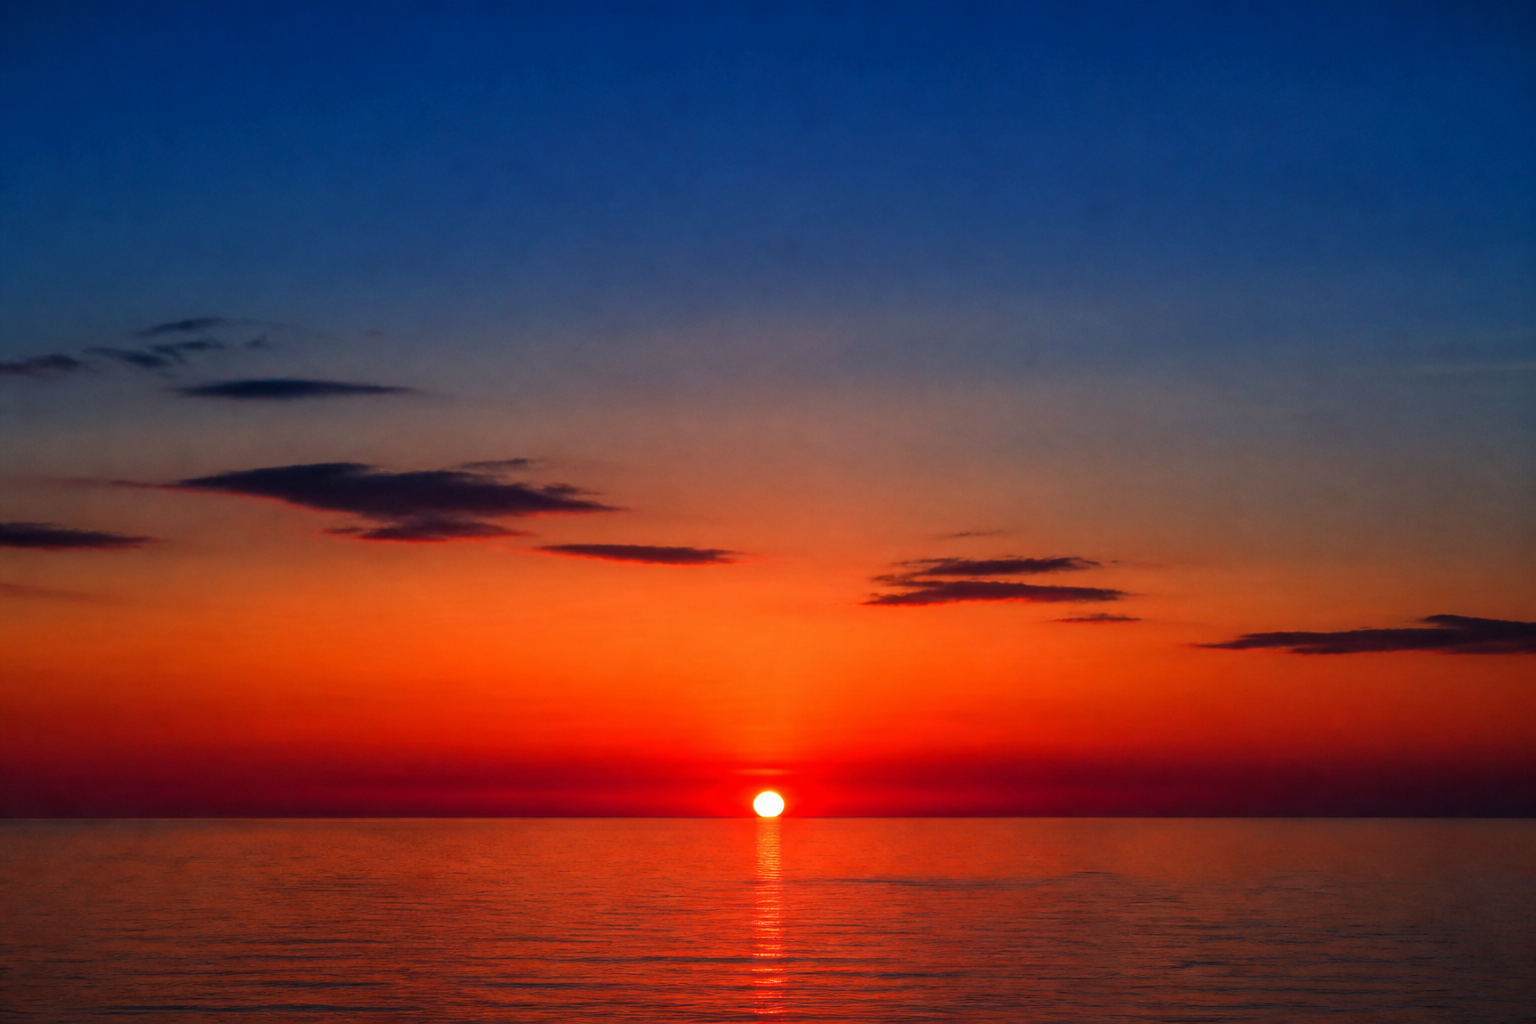
\includegraphics[width=0.58\linewidth]{images/book5/ai/b5-13-red-sunset.png}

{\small La puesta de sol como \omterm{thm:b3:perturbation-theory:corrections}{teoría de perturbaciones}: las moléculas del aire dispersan la luz azul mucho más fácilmente que la roja (el $\omega^4$ emparentado con la regla de oro de este capítulo), de modo que el largo camino del horizonte cuela el azul y se lo envía por correo al mediodía de otra persona.}
\end{omfigure}

\section{Ejercicios}

\begin{exercise}[$\star$]\label{exo:b3:perturbation-theory:1}
Una partícula en una caja $[0, a]$ siente el potencial adicional $V(x) =
\lambda x/a$. (a) Calcúlese el desplazamiento de primer orden de todos los
niveles (úsese $\langle x\rangle = a/2$ en cualquier estado de la caja ---
justifíquese). (b) ¿Por qué es aquí el mismo desplazamiento para todos los
niveles? (c) ¿Cuál es el cambio de primer orden de los \emph{espaciados}, y
por qué podría una medida de frecuencias de transición pasar por alto esta
perturbación por completo? (d) ¿Cuándo deja de ser fiable el primer orden?
\end{exercise}

\begin{exercise}[$\star$]\label{exo:b3:perturbation-theory:2}
Realícese por completo el cálculo de segundo orden de la
\cref{prop:b3:perturbation-theory:oscillator-field}: elementos de matriz
de $\hat x$, los dos términos, la cancelación de $n$ y
la coincidencia exacta con el resultado de completar el cuadrado. ¿Por qué
no se anula la corrección de primer orden del \emph{estado} aunque sí lo
hágase la de la energía?
\end{exercise}

\begin{exercise}[$\star$]\label{exo:b3:perturbation-theory:3}
El \omterm{def:b3:hamiltonian-mechanics:hamiltonian}{hamiltoniano} de dos niveles $\begin{pmatrix}E_1 & v\\ v &
E_2\end{pmatrix}$, con $E_1 < E_2$ y $v$ real. (a) Hállense los \omterm{def:b3:quantum-formalism:observable}{valores
propios} exactos. (b) Desarróllese para $|v| \ll E_2 - E_1$ e identifíquese la
fórmula de segundo orden. (c) Muéstrese que los niveles se repelen: la
separación supera siempre a $E_2 - E_1$. (d) En $E_1 = E_2$: ¿qué da la
\omterm{thm:b3:perturbation-theory:corrections}{teoría de perturbaciones}, qué da la respuesta exacta y qué teorema del
capítulo los reconcilia?
\end{exercise}

\begin{exercise}[$\star$]\label{exo:b3:perturbation-theory:4}
Para el \cref{thm:b3:perturbation-theory:corrections}: (a) muéstrese que la
corrección de primer orden del estado es ortogonal a $\ket n$; (b) muéstrese
que el coeficiente de mezcla de $\ket m$ es $V_{mn}/(E_n - E_m)$ y
enúnciese el criterio de validez; (c) un nivel situado a $\qty{1}{eV}$ de su
vecino más próximo está acoplado a él por \qty{0.1}{eV}: estímese la
probabilidad de mezcla; (d) lo mismo con una separación de \qty{10}{meV}:
¿qué herramienta debería sustituir al desarrollo?
\end{exercise}

\begin{exercise}[$\star\star$]\label{exo:b3:perturbation-theory:5}
Enlaces anarmónicos. Añádase $\hat V = \beta\hat x^3 + \gamma\hat x^4$ al
oscilador. (a) Muéstrese que el término en $x^3$ no desplaza ningún nivel a
primer orden (paridad). (b) Muéstrese que el término en $x^4$ da $\Delta E_n =
3\gamma(\hbar/2m\omega)^2(2n^2 + 2n + 1)$ (desarróllese $\hat x^4$ en
\omterm{def:b3:harmonic-oscillator:ladder}{operadores escalera}; solo sobreviven los términos ``equilibrados''). (c) Para un enlace real, el $\gamma$ efectivo es negativo (el pozo se
ablanda hacia fuera): muéstrese que el espaciado de niveles \emph{disminuye}
entonces con $n$.
(d) ¿Qué rasgo observado de los espectros moleculares
(\cref{exo:b3:harmonic-oscillator:4}) reproduce esto?
\end{exercise}

\begin{exercise}[$\star\star$]\label{exo:b3:perturbation-theory:6}
En la caja cuadrada bidimensional, la pareja degenerada $\ket{1,2},
\ket{2,1}$ se perturba con $\hat V = \lambda\,xy$. (a) Explíquese por qué
falla la teoría no degenerada. (b) Calcúlese la matriz $2\times2$ de
$\hat V$ en la pareja (las integrales se factorizan; $\int_0^a
x\sin(\pi x/a)\sin(2\pi x/a)\dd x = -8a^2/9\pi^2$). (c) Hállense los
desdoblamientos y los estados correctos de orden cero. (d) Compárese con
el análisis de simetría del \cref{exo:b3:quantum-formalism:9}: ¿qué
respuesta dio la simetría de balde?
\end{exercise}

\begin{exercise}[$\star\star$]\label{exo:b3:perturbation-theory:7}
\omterm{ex:b3:perturbation-theory:stark}{Efectos Stark}, lineal y cuadrático. (a) Usando el
\cref{ex:b3:perturbation-theory:stark}, calcúlese el desdoblamiento de
$n = 2$ en $\mathcal E = \qty{2.5e6}{V/m}$. (b) ¿Por qué \emph{no} muestra
desplazamiento lineal el estado fundamental (dos razones: la paridad y la
ausencia de compañero degenerado)? (c) Su desplazamiento cuadrático define
la polarizabilidad, $\Delta E = -\tfrac12\alpha\mathcal E^2$: estímense
$\alpha \sim e^2a_0^2/E_{\text{I}}$ y evalúese en unidades de
$a_0^3$ (la respuesta exacta es $4.5\,a_0^3 \times
4\pi\varepsilon_0$). (d) ¿De qué propiedad cotidiana de la materia ---
su respuesta dieléctrica --- acaba de calcular la semilla atómica?
\end{exercise}

\begin{exercise}[$\star\star$]\label{exo:b3:perturbation-theory:8}
Emisión espontánea (con un dato admitido): un estado excitado se
desintegra con $A = \omega^3|d_{fi}|^2/3\pi\varepsilon_0\hbar c^3$,
donde elementos de matriz del tipo $d_{fi} = e\bra f\hat z\ket i$ fijan el
dipolo. (a) Para el $2p \to 1s$ del hidrógeno: con $|d| \approx 0.74\,
ea_0$ y $\lambda = \qty{121.6}{nm}$, calcúlense $A$ y la
vida media. (b) Escálese a la línea D del sodio. (c) Escálese a la
transición hiperfina de 21 cm ($|d| \to$ un momento magnético, con el ritmo
rebajado en otro factor del orden de $\alpha^2$; acéptese $A \approx
\qty{2.9e-15}{s^{-1}}$): compruébense los ``diez millones de años''. (d)
A partir del $\omega^3$: ¿por qué son rápidas las líneas ultravioletas y
eternas las de radio, y por qué hizo eso a la \omterm{ex:b3:spin-two-level:hyperfine}{línea de 21 cm}
\emph{predecible} pero casi indetectable en un laboratorio?
\end{exercise}

\begin{exercise}[$\star\star$]\label{exo:b3:perturbation-theory:9}
Reglas de selección como integrales. (a) Muéstrese que $\bra{100}\hat z\ket{200} =
0$ por paridad. (b) Muéstrese que $\bra{100}\hat z\ket{21m} = 0$ salvo si $m =
0$ (la integral en $\varphi$). (c) Enúnciense las reglas resultantes $\Delta
l = \pm1$, $\Delta m = 0, \pm1$ y su lectura física (el espín del
fotón). (d) El estado $2s$ no puede alcanzar el $1s$ por ninguna vía
dipolar: ¿qué predice eso para su vida media y qué camino ``prohibido'' de
dos fotones toma en realidad la naturaleza?
\end{exercise}

\begin{exercise}[$\star\star\star$]\label{exo:b3:perturbation-theory:10}
Polarizabilidad, con honradez. El desplazamiento de segundo orden del estado
fundamental del hidrógeno en un campo es $\Delta E = -e^2\mathcal E^2\sum_{m\neq
0}|\bra m\hat z\ket 0|^2/(E_m - E_0)$. (a) Acótese la suma
sustituyendo todos los denominadores por la separación mínima $E_2 - E_1 =
\tfrac34 E_{\text{I}}$ y usando la relación de cierre $\sum_m|\bra
m\hat z\ket0|^2 = \langle z^2\rangle_0 = a_0^2$: obténgase $\alpha
\le \tfrac{16}3\,a_0^3$ (en unidades de estilo gaussiano de
$4\pi\varepsilon_0$). (b) Compárese con el valor exacto $\tfrac92 a_0^3$.
(c) A partir de $\alpha$, estímese el índice de refracción del hidrógeno
gaseoso a densidad atmosférica ($n - 1 \approx N\alpha/2\varepsilon_0
\cdot e^2\dots$ --- úsese $n - 1 = N\alpha_{\text{SI}}/2
\varepsilon_0$) y compárese con el valor medido $\num{1.3e-4}$.
(d) Enúnciese en una frase la cadena átomo $\to$ polarizabilidad
$\to$ refracción que cabalgará la parte II del problema de fin de semana.
\end{exercise}

\begin{exercise}[$\star\star\star$]\label{exo:b3:perturbation-theory:11}
Cruces evitados y barridos lentos. Un sistema de dos niveles tiene energías
desnudas $\pm\lambda t$ que se cruzan en $t = 0$, acopladas por $v$. (a)
Esbócense los niveles exactos frente a $t$: un cruce evitado de separación
$2|v|$. (b) Si el barrido es \emph{lento}, el sistema sigue la curva
inferior (teorema adiabático, admitido): ¿en qué estado acaba? (c) El
criterio de Landau--Zener compara el tiempo de barrido a través de la región
de la separación, $\sim v/\lambda$, con el reloj interno
$\hbar/v$: dese la condición de seguimiento adiabático. (d) Dos
aplicaciones: el estado de un cúbit transferido por un barrido lento de
frecuencia; una colisión atómica que salta carga entre núcleos --- explíquese
una de ellas en dos frases.
\end{exercise}

\begin{exercise}[$\star\star\star$]\label{exo:b3:perturbation-theory:12}
El segundo orden es pesimista, y otros teoremas. (a) Muéstrese que
la corrección de segundo orden al estado \emph{fundamental} es siempre
negativa. (b) Conclúyase (con el
\cref{exo:b3:harmonic-oscillator:10}) por qué las fuerzas de van der Waals
son siempre atractivas entre átomos en su estado fundamental. (c) Muéstrese
que la teoría de primer orden \emph{sobrestima} toda energía del estado
fundamental: es una cota variacional (evalúese $\bra{\psi_0}\hat
H\ket{\psi_0}$ con el estado sin perturbar como función de prueba). (d) Una
comprobación de coherencia sobre el \cref{ex:b3:perturbation-theory:stark}:
¿por qué no viola el \omterm{ex:b3:perturbation-theory:stark}{efecto Stark} \emph{lineal} el apartado (a)?
\end{exercise}

\section{Problema: el color del cielo}

\begin{problem}[{Problema de fin de semana --- la dispersión de Rayleigh
por átomos perturbados}]\label{pb:b3:perturbation-theory:1}
¿Por qué es azul el cielo diurno, roja la puesta de sol y blanca la nube? La
respuesta completa es una cadena que atraviesa este capítulo: una onda
luminosa perturba cada molécula del aire; el dipolo inducido vuelve a radiar
(la radiación dipolar del volumen del Año 2); y la interferencia decide qué
sobrevive. Datos: polarizabilidad molecular del aire
$\alpha/4\pi\varepsilon_0 \approx \qty{2.2e-30}{m^3}$; densidad
numérica $N = \qty{2.5e25}{m^{-3}}$; rango visible
$450$--\qty{700}{nm}.

\medskip\noindent\textbf{Parte I --- La molécula perturbada.}
\begin{enumerate}
  \item Un campo estático $\mathcal E$ desplaza el estado fundamental de
        una molécula en $-\tfrac12\alpha\mathcal E^2$: conéctese este
        enunciado con la \omterm{thm:b3:perturbation-theory:corrections}{teoría de perturbaciones} de segundo orden (¿qué
        fórmula y por qué negativo?).
  \item El mismo $\alpha$ da el dipolo inducido $p =
        \alpha\mathcal E$: para el campo de la luz solar $\mathcal E \sim
        \qty{800}{V/m}$, calcúlese el dipolo inducido de una molécula de
        nitrógeno y compárese con $ea_0$.
  \item ¿Por qué puede tratarse el campo óptico (de frecuencia
        $\num{5e14}$ Hz) con la polarizabilidad \emph{estática} en el caso
        de moléculas cuyas transiciones electrónicas caen en el
        ultravioleta? (Compárese $\hbar\omega$ con la separación; este es el
        límite muy fuera de resonancia del denominador de la regla de
        oro).
  \item Un dipolo oscilante $p_0\cos\omega t$ radia la potencia media
        $P = p_0^2\omega^4/12\pi\varepsilon_0c^3$
        (volumen del Año 2). Combinándolo con $p_0 = \alpha\mathcal
        E_0$: ¿cómo depende de $\omega$ la potencia dispersada a
        iluminación fija?
  \item Calcúlese la razón de potencias dispersadas a \qty{450}{nm}
        y a \qty{700}{nm}.
  \item En una frase: ¿por qué es el cielo azul y no violeta
        (dos ingredientes: el espectro del Sol, que decae hacia el
        violeta, y la sensibilidad del ojo)?
\end{enumerate}

\medskip\noindent\textbf{Parte II --- De una molécula al
cielo.}
\begin{enumerate}[resume]
  \item La sección eficaz de dispersión resulta ser $\sigma =
        \dfrac{8\pi}{3}\Big(\dfrac{\alpha}{4\pi\varepsilon_0}
        \Big)^2\dfrac{\omega^4}{c^4}$: verifíquense sus dimensiones y
        evalúese a \qty{550}{nm}.
  \item La longitud de atenuación es $\ell = 1/N\sigma$: evalúese
        a \qty{550}{nm} y compárese con el espesor de la
        atmósfera ($\sim\qty{8}{km}$ equivalentes a densidad del nivel
        del mar).
  \item A \qty{450}{nm} frente a \qty{700}{nm}, ¿qué fracción de un haz
        solar vertical se dispersa hacia fuera? (Úsese $1 -
        \eu^{-L/\ell}$ con $L = \qty{8}{km}$).
  \item En la puesta de sol el camino es treinta veces más largo: recalcúlese
        la supervivencia del azul y explíquense el color del Sol bajo ---
        y el de la luz que enrojece la Luna en un eclipse
        lunar.
  \item ¿Por qué está \emph{polarizada} la luz del cielo a $90^\circ$
        del Sol (recuérdese el diagrama de radiación dipolar: no hay
        emisión a lo largo del eje del dipolo)?
  \item Se dice que las abejas y los vikingos navegaban con esa
        polarización: ¿qué le hace un día nublado, y por qué?
\end{enumerate}

\medskip\noindent\textbf{Parte III --- Por qué no brilla más el
cielo.}
\begin{enumerate}[resume]
  \item Una paradoja: en un medio perfectamente uniforme, las ondículas
        de elementos de volumen vecinos interfieren destructivamente hacia
        los lados y \emph{no} se dispersaría luz alguna (solo sobreviviría
        la refracción). ¿Qué rompe realmente la uniformidad del aire, es
        decir, qué está distribuido al azar?
  \item Las fluctuaciones de densidad de un gas ideal hacen que las
        intensidades dispersadas por moléculas independientes \emph{se
        sumen}: dígase por qué la independencia (posiciones al azar,
        separaciones de escala de la longitud de onda) mata la
        interferencia destructiva.
  \item A partir de su $\ell$ a \qty{550}{nm}: ¿qué fracción de la
        luz solar dispersa una atmósfera en un día despejado? ¿Casa
        el número con el brillo cotidiano del cielo frente al Sol?
  \item Una gotita de nube (\qty{10}{\micro m}) contiene $\sim10^{12}$
        moléculas dentro de una longitud de onda: sus ondículas se suman
        \emph{coherentemente}. ¿Cómo escala entonces la potencia
        dispersada con el número de moléculas, y por qué desaparece la
        selección de color por $\omega^4$ (todas las longitudes de onda
        se dispersan con fuerza)? ¿De qué color es la nube?
  \item La leche, la niebla y la pintura blanca son blancas por la misma
        razón: enúnciese la regla general --- los dispersores pequeños
        frente a $\lambda$ colorean la luz y los grandes frente a
        $\lambda$ la blanquean.
  \item Opalescencia crítica: cerca del punto crítico de un líquido
        (los capítulos de cambio de fase del volumen del Año 1 y el
        \cref{ch:b3:phase-transitions} que viene), las fluctuaciones de densidad crecen hasta escalas ópticas y
        el fluido se vuelve lechoso: conéctese con el apartado 13.
\end{enumerate}

\medskip\noindent\textbf{Parte IV --- La cadena, completada.}
\begin{enumerate}[resume]
  \item Las ondículas dispersadas hacia delante \emph{no} se cancelan:
        interfieren con el haz y frenan su fase --- el
        índice de refracción. Usando $n - 1 = N\alpha/2\varepsilon_0$
        (con $\alpha$ en unidades SI), evalúese $n - 1$ para el aire y
        compárese con el valor medido \num{2.9e-4}.
  \item Una sola constante $\alpha$, calculada por \omterm{thm:b3:perturbation-theory:corrections}{teoría de
        perturbaciones} de segundo orden, fija así tres fenómenos a la vez:
        nómbrelos (el desplazamiento en un campo estático, el azul del
        cielo y la desviación de la luz en el aire).
  \item La absorción del ozono, los aerosoles y la dispersión múltiple
        complican los cielos reales: nómbrese un observable de cada uno
        (los colores del crepúsculo; el horizonte lechoso; el brillo
        residual del cielo en el cenit tras la puesta de sol).
  \item ¿Por qué tiene la Luna, sin aire, un cielo diurno \emph{negro}
        --- y qué confirmó así toda fotografía tomada desde su superficie
        sobre el origen del nuestro?
  \item El cielo diurno de Marte es color caramelo y sus puestas de sol
        son \emph{azules}: su aire tenue dispersa poco y el trabajo lo
        hacen granos de polvo de micrómetros en suspensión. Usando la
        regla del apartado 18, explíquese cómo invierte el polvo la lógica
        del color.
  \item Para los rayos X, $\hbar\omega$ supera con creces toda transición
        molecular: los electrones responden como si fueran libres y la
        dispersión (Thomson) pierde su $\omega^4$. ¿Qué le ocurre al
        mecanismo del ``azul del cielo'' en ese régimen, y por qué es esa
        respuesta plana precisamente lo que hace de los rayos X sondas
        limpias de la densidad electrónica?
  \item Resúmase el resultado con nombre propio: una polarizabilidad de
        $\qty{2.2e-30}{m^3}$, elevada al cuadrado y multiplicada por
        $\omega^4$, da una longitud de dispersión de escala \qty{60}{km}
        en el verde --- lo bastante larga para que el cielo del mediodía
        sea suave y lo bastante corta para que las puestas de sol
        enrojezcan y los cielos sean azules, con el patrón de polarización
        de un bosque de dipolos excitados.
\end{enumerate}
\end{problem}
